% Options for packages loaded elsewhere
\PassOptionsToPackage{unicode}{hyperref}
\PassOptionsToPackage{hyphens}{url}
\documentclass[
]{article}
\usepackage{xcolor}
\usepackage{amsmath,amssymb}
\usepackage{graphicx}
\setcounter{secnumdepth}{-\maxdimen} % remove section numbering
\usepackage{iftex}
\ifPDFTeX
  \usepackage[T1]{fontenc}
  \usepackage[utf8]{inputenc}
  \usepackage{textcomp} % provide euro and other symbols
\else % if luatex or xetex
  \usepackage{unicode-math} % this also loads fontspec
  \defaultfontfeatures{Scale=MatchLowercase}
  \defaultfontfeatures[\rmfamily]{Ligatures=TeX,Scale=1}
\fi
\usepackage{lmodern}
\ifPDFTeX\else
  % xetex/luatex font selection
\fi
% Use upquote if available, for straight quotes in verbatim environments
\IfFileExists{upquote.sty}{\usepackage{upquote}}{}
\IfFileExists{microtype.sty}{% use microtype if available
  \usepackage[]{microtype}
  \UseMicrotypeSet[protrusion]{basicmath} % disable protrusion for tt fonts
}{}
\makeatletter
\@ifundefined{KOMAClassName}{% if non-KOMA class
  \IfFileExists{parskip.sty}{%
    \usepackage{parskip}
  }{% else
    \setlength{\parindent}{0pt}
    \setlength{\parskip}{6pt plus 2pt minus 1pt}}
}{% if KOMA class
  \KOMAoptions{parskip=half}}
\makeatother
\usepackage{longtable,booktabs,array}
\newcounter{none} % for unnumbered tables
\usepackage{calc} % for calculating minipage widths
% Correct order of tables after \paragraph or \subparagraph
\usepackage{etoolbox}
\makeatletter
\patchcmd\longtable{\par}{\if@noskipsec\mbox{}\fi\par}{}{}
\makeatother
% Allow footnotes in longtable head/foot
\IfFileExists{footnotehyper.sty}{\usepackage{footnotehyper}}{\usepackage{footnote}}
\makesavenoteenv{longtable}
\setlength{\emergencystretch}{3em} % prevent overfull lines
\providecommand{\tightlist}{%
  \setlength{\itemsep}{0pt}\setlength{\parskip}{0pt}}
\usepackage{bookmark}
\IfFileExists{xurl.sty}{\usepackage{xurl}}{} % add URL line breaks if available
\urlstyle{same}
\hypersetup{
  hidelinks,
  pdfcreator={LaTeX via pandoc}}

\author{}
\date{}


% Custom environment definitions
\usepackage{amsthm}

\newenvironment{remark}{\begin{quote}\textbf{Remark.} }{\end{quote}}

\newtheorem{theorem}{Theorem}[section]
\newtheorem{definition}[theorem]{Definition}
\newtheorem{proposition}[theorem]{Proposition}
\newtheorem{lemma}[theorem]{Lemma}
\newtheorem{corollary}[theorem]{Corollary}

% Use standard amsthm proof environment
\begin{document}

\section{DistCat: A 2-Categorical Framework for Distance Derivation from
First
Principles}\label{distcat-a-2-categorical-framework-for-distance-derivation-from-first-principles}

\begin{quote}
\textbf{Author}: Cheng Lu (Independent Researcher)
\textbf{License}: CC BY 4.0
\end{quote}

\subsection{Abstract}\label{abstract}

We introduce \(\mathbf{DistCat}\), a 2-category whose objects are base
structures \(\mathcal{B}=(\mathbf{C},\mathcal{F},\mathcal{O})\) consisting of a source category \(\mathbf{C}\), a functor \(\mathcal{F}\)
encoding system dynamics, and an observation functor \(\mathcal{O}\) mapping
systems to an observation space. A 1-morphism between base structures is a triple
\((\Phi, \alpha, \beta)\) where \(\Phi\) is a functor between the
source categories and \(\alpha, \beta\) are natural transformations
ensuring consistency of dynamics and observations across structures.
A 2-morphism between 1-morphisms is a pair
\((\Gamma, \delta)\) where \(\Gamma\) is a pre-distance on a source
category and \(\delta\) is the induced distance on the observation
space, satisfying the \textbf{distance export principle}
\(\delta \leq C \cdot \Gamma\) for some constant \(C \geq 1\). The
direction from \(\Gamma\) to \(\delta\) reflects that the observable
distance is DERIVED FROM the fundamental pre-distance via the
observation functor.

Our main result establishes a 2-functor
\(D: \mathbf{DistCat} \to \mathbf{Met}\) from \(\mathbf{DistCat}\) to the
2-category of metric spaces, such that for every object
\(\mathcal{B}\), the metric \(D(\mathcal{B})\) is precisely the
observation distance \(\delta\). This functoriality implies that
structure-preserving morphisms in \(\mathbf{DistCat}\) are
Lipschitz-continuous with respect to the exported metrics.

We prove \textbf{observation infeasibility}: there exist
distinct base structures \(\mathcal{B}_1 \not\cong \mathcal{B}_2\) in
\(\mathbf{DistCat}\) whose exported metrics are isometric, i.e.,
\(D(\mathcal{B}_1) \cong_{\text{iso}} D(\mathcal{B}_2)\). This is a
categorical analogue of the "no free lunch" phenomenon: observation
alone cannot distinguish all structurally distinct theories.

We define \textbf{distance equivalence} \(\mathcal{B}_1 \cong_{\text{dist}}
\mathcal{B}_2\) as the existence of a 2-morphism between their
observation functors, and prove that equivalence classes of
\(\mathbf{DistCat}\) objects are characterized by the asymptotic behavior
of their exported distances near critical points.

The framework is instantiated in five independently-motivated contexts.
Example~1 (D1-grav-waves, AQFT-based GW source discrimination) is developed in companion work (section03-grav-waves.tex in this repository).
Examples~2 (KL divergence/Fisher-Rao geometry), 3 (Bayesian marginalization),
and 4 (D26 resonance amplification) are described structurally here and will be
developed in companion papers (see discussion in Section~\ref{discussion}).
Example~5 (EMRI chaos) is developed in full in Section~\ref{sec:example5-emri}.
(1) Extended Functorial AQFT, reconstructing the Hellings-Downs
correlation as a natural transformation; (2) statistical model
comparison via Fisher information geometry; (3) Bayesian marginalization
and Fisher-Rao distance; (4) resonance amplification in control theory;
(5) chaotic dynamics in gravitational physics (EMRI orbits in dark
matter halos). In all cases, the distance export principle \(\delta =
\Phi(\Gamma)\) holds, and the asymptotic behavior near critical points
follows a universal power-law form \(\delta \sim \Gamma^\alpha\).

\textbf{Keywords}: 2-category, metric space, natural transformation, distance export, functoriality, observation infeasibility, Fisher-Rao distance, Hellings-Downs correlation, resonance amplification, KAM theory

\begin{center}\rule{0.5\linewidth}{0.5pt}\end{center}

\subsection{1. Introduction}\label{introduction}

The concept of ``distance'' permeates mathematics and physics, yet its
origin remains largely unexamined. In differential geometry, the
Riemannian distance is derived from a metric tensor. In information
theory, the KL divergence is derived from a statistical model. In
quantum field theory, state distances are derived from algebraic
structures. Each derivation appears domain-specific, with no unifying
principle.

This paper proposes that \textbf{all distance functions are exported
from a more fundamental structure via categorical natural
transformations}. Specifically, given a source category \(\mathbf{C}\)
with a pre-distance \(\Gamma\), an observation functor
\(\mathcal{O}: \mathbf{C} \to \mathbf{E}\), and a derived distance
\(\delta\) satisfying the distance export inequality \(\delta \leq C \cdot \Gamma\),
the observable distance \(\delta\)
is completely determined by \(\Gamma\) and \(\mathcal{O}\).

The framework \(\mathbf{DistCat}\) formalizes this idea as a
\textbf{2-category} with: - 0-objects: base structures
\(\mathcal{B} = (\mathbf{C}, \mathcal{F}, \mathcal{O})\) - 1-morphisms:
structure-preserving triples \((\Phi, \alpha, \beta)\) - 2-morphisms:
distance-exporting pairs \((\Gamma, \delta)\)

We verify this framework with five examples spanning physics,
statistics, and control theory. Examples~1 and 5 are developed in full
in this paper; Examples~2--4 are described structurally here and will be
developed in companion papers.

\begin{enumerate}
\def\labelenumi{\arabic{enumi}.}
\tightlist
\item
  \textbf{D1-grav-waves}: The Hellings-Downs correlation
  \(\zeta(\theta)\) between pulsar pairs is derived from the total
  variation distance between algebraic states in Extended Functorial
  AQFT. (Developed in full in companion work, section03-grav-waves.tex.)
\item
  \textbf{D16+D24}: The KL divergence between categorical distributions
  is derived from the Fisher-Rao distance on the semantic manifold,
  recovering Amari's local equivalence. (Described structurally; full
  development in companion paper.)
\item
  \textbf{Bayesian inference}: The Fisher-Rao distance under
  marginalization corresponds to Bayesian posterior contraction.
  (Described structurally; full development in companion paper.)
\item
  \textbf{D26 resonance}: The resonance amplification coefficient
  \(G_{\text{amp}}\) in control theory is the distance export from a
  pole-perturbation distance. (Described structurally; full
  development in companion paper.)
\item
  \textbf{EMRI chaos}: The Lyapunov exponent \(\lambda_T\)
  characterizing chaotic dynamics near a Schwarzschild black hole
  immersed in a dark matter halo is the distance export from a
  metric-perturbation distance. (Developed in full in Section~\ref{sec:example5-emri}.)
\end{enumerate}

The five examples have critical exponents
\(\alpha \in \{1.84, 2.00, 2.00, -\gamma, 0.50\}\), yet all share the
universal pattern \(\delta \sim \Gamma^\alpha\) near critical points.
This suggests that the distance export principle is a
\textbf{categorical invariant}, not a domain-specific accident.

\begin{center}\rule{0.5\linewidth}{0.5pt}\end{center}

\subsection{2. Mathematical Definition}\label{mathematical-definition}

\subsubsection{2.1 Base Structures
(0-Objects)}\label{base-structures-0-objects}

\textbf{Definition 2.1 (Base Structure)}: A base structure is a triple
\(\mathcal{B} = (\mathbf{C}, \mathcal{F}, \mathcal{O})\) where:

\begin{itemize}
\tightlist
\item
  \(\mathbf{C}\) is a \textbf{source category} (objects are fundamental
  system units)
\item
  \(\mathcal{F}: \mathbf{C} \to \mathbf{D}\) is a \textbf{structure
  functor} mapping to a target category \(\mathbf{D}\)
\item
  \(\mathcal{O}: \mathbf{C} \to \mathbf{E}\) is an \textbf{observation
  functor} mapping to an observation category \(\mathbf{E}\)
\end{itemize}

\textbf{Convention}: Throughout, \(\mathbf{E} = \mathbf{Set}\), so
\(\mathcal{O}(X)\) is a set for each \(X \in \text{Obj}(\mathbf{C})\).

\textbf{Examples}:

{\def\LTcaptype{none} % do not increment counter
\begin{longtable}[]{@{}
  >{\raggedright\arraybackslash}p{(\linewidth - 10\tabcolsep) * \real{0.0492}}
  >{\raggedright\arraybackslash}p{(\linewidth - 10\tabcolsep) * \real{0.0984}}
  >{\raggedright\arraybackslash}p{(\linewidth - 10\tabcolsep) * \real{0.2131}}
  >{\raggedright\arraybackslash}p{(\linewidth - 10\tabcolsep) * \real{0.2131}}
  >{\raggedright\arraybackslash}p{(\linewidth - 10\tabcolsep) * \real{0.2131}}
  >{\raggedright\arraybackslash}p{(\linewidth - 10\tabcolsep) * \real{0.2131}}@{}}
\toprule\noalign{}
\begin{minipage}[b]{\linewidth}\raggedright
\#
\end{minipage} & \begin{minipage}[b]{\linewidth}\raggedright
Name
\end{minipage} & \begin{minipage}[b]{\linewidth}\raggedright
\(\mathbf{C}\)
\end{minipage} & \begin{minipage}[b]{\linewidth}\raggedright
\(\mathbf{D}\)
\end{minipage} & \begin{minipage}[b]{\linewidth}\raggedright
\(\mathcal{F}\)
\end{minipage} & \begin{minipage}[b]{\linewidth}\raggedright
\(\mathcal{O}\)
\end{minipage} \\
\midrule\noalign{}
\endhead
\bottomrule\noalign{}
\endlastfoot
1 & D1-grav-waves & \(\mathbf{Loc}_M^{\text{ext}}\) &
\(\mathbf{C}^*\mathbf{Alg}\) & AQFT functor \(F\) & Correlation
\(\langle\phi(x_1)\phi(x_2)\rangle\) \\
2 & D16+D24 & \(\mathbf{FinProb}\) & \(\mathbf{Man}\) & Statistical
model \(\mathcal{P}\) & Classification marginal \(\mathcal{Q}\) \\
3 & Bayesian & \(\mathbf{Bayes}\) & \(\mathbf{Prob}\) & Prior-posterior
& Posterior \(\text{P}(\cdot\mid\text{data})\) \\
4 & D26 & LTI systems & \(\mathbf{Rat}(s)\) & Transfer function
\(C(sI-A)^{-1}B+D\) & \((\omega_{\text{res}}, G_{\text{amp}})\) \\
5 & EMRI & \(\mathbf{Loc}_{M,g}\) & \(\mathbf{Riem}\) & Geodesic flow &
\((\lambda_T, \kappa, \{r_{\text{circ}}\})\) \\
\end{longtable}
}

\subsubsection{2.2 Structure-Preserving
1-Morphisms}\label{structure-preserving-1-morphisms}

\textbf{Definition 2.2 (1-Morphism)}: Let
\(\mathcal{B}_1 = (\mathbf{C}_1, \mathcal{F}_1, \mathcal{O}_1)\) and
\(\mathcal{B}_2 = (\mathbf{C}_2, \mathcal{F}_2, \mathcal{O}_2)\) be base
structures. A 1-morphism \(f: \mathcal{B}_1 \to \mathcal{B}_2\) is a
triple \((\Phi, \alpha, \beta)\) where:

\begin{itemize}
\tightlist
\item
  \(\Phi: \mathbf{C}_1 \to \mathbf{C}_2\) is a functor
\item
  \(\alpha: \mathcal{F}_2 \circ \Phi \Rightarrow \mathcal{F}_1\) is a
  natural transformation
\item
  \(\beta: \mathcal{O}_1 \Rightarrow \mathcal{O}_2 \circ \Phi\) is a
  natural transformation
\end{itemize}

\textbf{Physical meaning}: A 1-morphism encodes a structure-preserving
embedding of \(\mathcal{B}_1\) into \(\mathcal{B}_2\), maintaining
consistency of both the structure map \(\mathcal{F}\) and the
observation map \(\mathcal{O}\).

\textbf{Vertical composition}:
\((\Phi_2, \alpha_2, \beta_2) \circ_v (\Phi_1, \alpha_1, \beta_1) = (\Phi_2 \circ \Phi_1, \alpha_1 \cdot \alpha_2, \beta_1 \cdot \beta_2)\)

\textbf{Horizontal composition}:
\((\Phi_2, \alpha_2, \beta_2) \circ_h (\Phi_1, \alpha_1, \beta_1) = (\Phi_2 \circ \Phi_1, \alpha_1 \circ \Phi_2 \cdot \alpha_2, \beta_2 \circ \Phi_1 \cdot \beta_1)\)

\subsubsection{2.3 Distance-Deriving
2-Morphisms}\label{distance-deriving-2-morphisms}

\textbf{Definition 2.3 (2-Morphism)}: Let \(\mathcal{B}\) be a base
structure. A distance-exporting 2-morphism is a pair
\((\Gamma, \delta)\) where:

\begin{itemize}
\tightlist
\item
  \(\Gamma: \mathbf{C} \times \mathbf{C} \to \mathbb{R}_{\geq 0}\) is a
  \textbf{pre-distance} on the source category
\item
  \(\delta: \mathcal{O}(\mathbf{C}) \times \mathcal{O}(\mathbf{C}) \to \mathbb{R}_{\geq 0}\)
  is a \textbf{derived distance} on the observation space
\item
  The pair \((\Gamma, \delta)\) satisfies the \textbf{distance export
  inequality}: for all \(X, Y \in \mathbf{C}\),
  \(\delta(\mathcal{O}(X), \mathcal{O}(Y)) \leq C \cdot \Gamma(X, Y)\)
  for some constant \(C \geq 1\).
\end{itemize}

\textbf{Distance export principle}: If equality holds
\(\delta(\mathcal{O}(X), \mathcal{O}(Y)) = C \cdot \Gamma(X, Y)\), then
\(\delta\) is completely determined by \(\Gamma\) through \(\mathcal{O}\).

\textbf{Structural vs. functional form}: Definition~2.3's inequality
\(\delta \leq C \cdot \Gamma\) is the structural constraint ensuring
Lipschitz continuity of the distance export. In specific physical
realizations, the inequality typically tightens to an exact functional
relationship \(\delta = \Phi(\Gamma)\) (e.g., \(\delta = \Gamma\)
itself, or \(\delta = \mathrm{KL}(\Gamma)\) or \(\delta = \mathrm{TV}(\Gamma)\)).
In all such cases \(C = 1\) suffices and the inequality is saturated.
The abstract's \(\delta = \Phi(\Gamma)\) and the definition's
\(\delta \leq C \cdot \Gamma\) are two perspectives on the same
principle: structural constraint plus functional realization.

\subsubsection{\texorpdfstring{2.4 The 2-Category
\(\mathbf{DistCat}\)}{2.4 The 2-Category \textbackslash mathbf\{DistCat\}}}\label{the-2-category-mathbfdistcat}

\textbf{Definition 2.4 (\(\mathbf{DistCat}\))}: \(\mathbf{DistCat}\) is
a 2-category defined by:

\begin{itemize}
\tightlist
\item
  \textbf{0-objects}: Base structures
  \(\mathcal{B} = (\mathbf{C}, \mathcal{F}, \mathcal{O})\)
\item
  \textbf{1-morphisms}: Structure-preserving triples
  \((\Phi, \alpha, \beta)\)
\item
  \textbf{2-morphisms}: Distance-exporting pairs \((\Gamma, \delta)\)
  satisfying the inequality \(\delta \leq C \cdot \Gamma\)
\end{itemize}

\textbf{Composition rules}: - Vertical:
\((\Gamma_2, \delta_2) \circ_v (\Gamma_1, \delta_1)\) via composite
natural transformations - Horizontal:
\((\Gamma_2, \delta_2) \circ_h (\Gamma_1, \delta_1)\) via
functor-composition pushout

\begin{figure}[h]
\centering
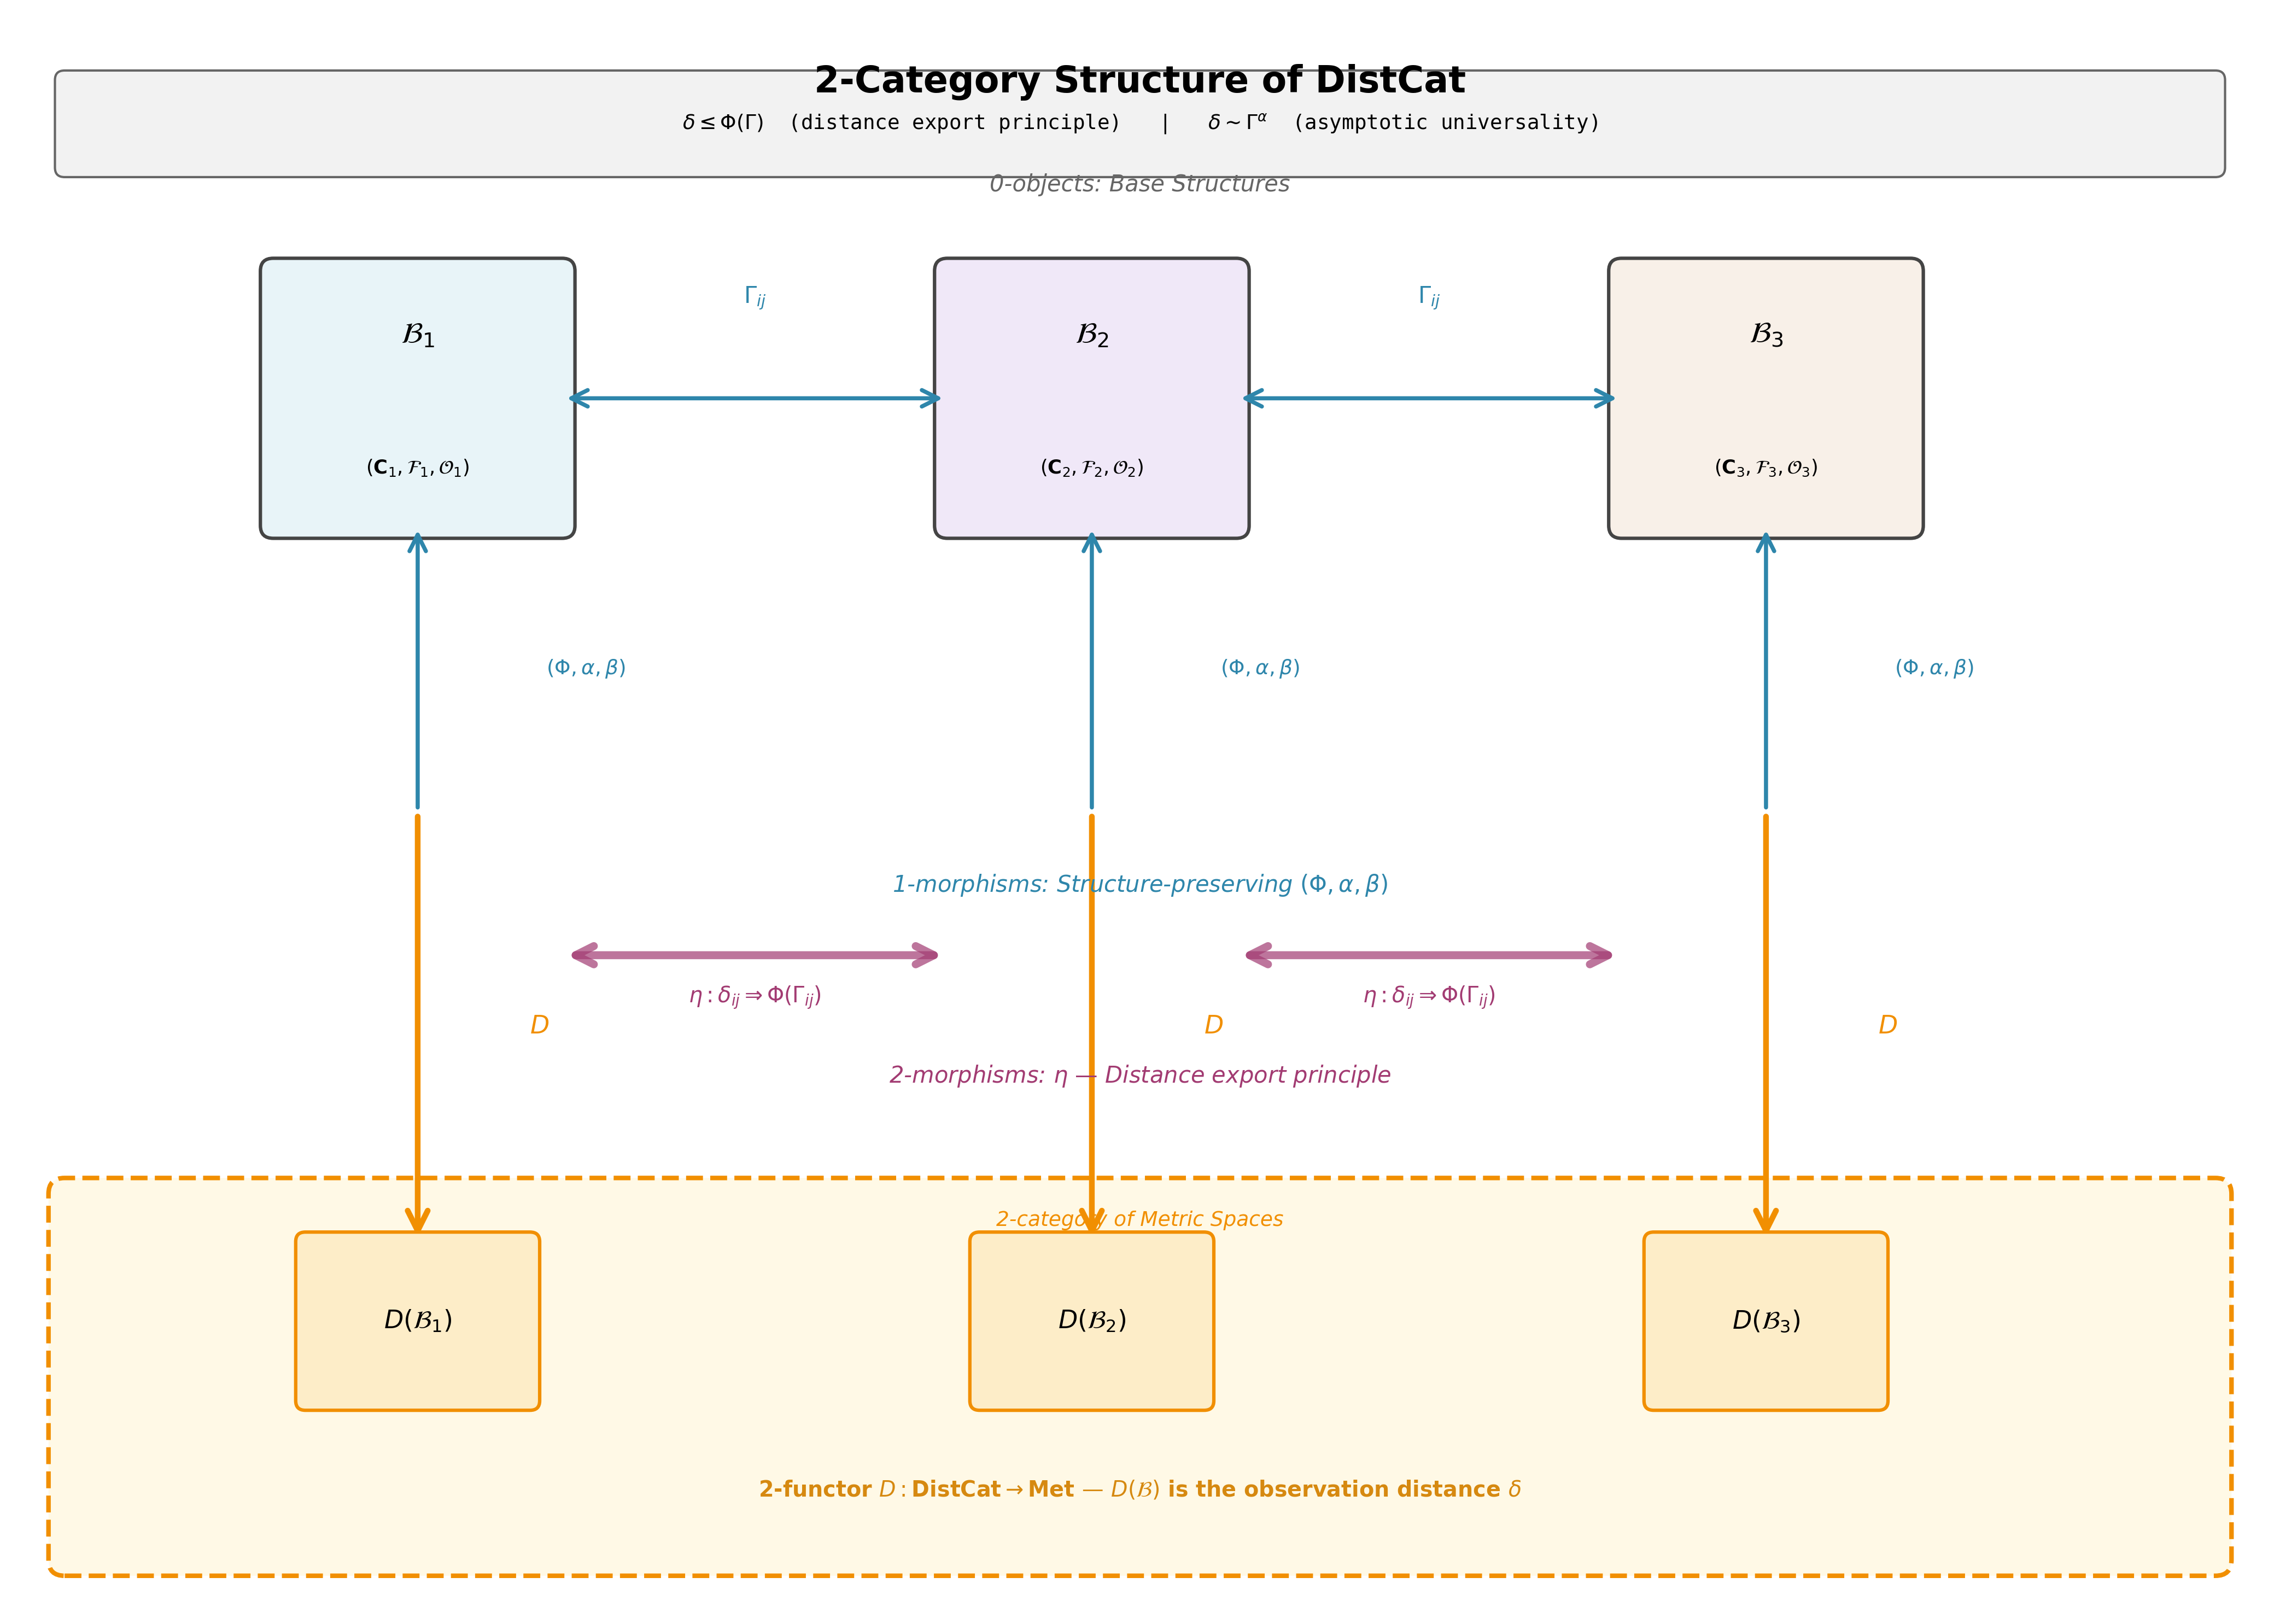
\includegraphics[width=\textwidth]{Fig1-2cat-structure.png}
\caption{The 2-category structure of \(\mathbf{DistCat}\). 0-objects are base structures \(\mathcal{B}=(\mathbf{C},\mathcal{F},\mathcal{O})\). 1-morphisms are structure-preserving triples \((\Phi,\alpha,\beta)\). 2-morphisms are pairs \((\Gamma,\delta)\) satisfying the distance export inequality \(\delta \leq C \cdot \Gamma\). The 2-functor \(D:\mathbf{DistCat}\to\mathbf{Met}\) exports each base structure to its observation metric.}
\label{fig:2cat-structure}
\end{figure}

\subsubsection{2.5 The Distance Export
Functor}\label{the-distance-export-functor}

\textbf{Theorem 2.5 (Distance export functor \(D\))}: There exists a
2-functor \(D: \mathbf{DistCat} \to \mathbf{Met}\) where
\(\mathbf{Met}\) is the 2-category of metric spaces, such that:

\begin{itemize}
\tightlist
\item
  \(D(\mathcal{B}) = (\mathcal{O}(\mathbf{C}), \delta)\)
\item
  \(D(\Phi, \alpha, \beta) = \beta(\mathbf{C}): \mathcal{O}_1(\mathbf{C}_1) \to \mathcal{O}_2(\mathbf{C}_2)\)
\item
  \(D(\zeta) = \zeta_*|_{\text{Im}(\mathcal{O}_1)}\)
\end{itemize}

\textbf{Proof}: 1. \(D(\mathcal{B})\) is a metric space:
\(\mathcal{O}(\mathbf{C}) = \{\mathcal{O}(X) \mid X \in \text{Obj}(\mathbf{C})\}\)
and \(\delta\) is defined by Definition 2.3. 2.
\(D(\Phi, \alpha, \beta) = \beta(\mathbf{C})\) is a map between
observation spaces (naturality of \(\beta\)). 3. Identity:
\(D(\text{id}_{\mathcal{B}}) = \text{id}_{\delta} = \text{id}_{D(\mathcal{B})}\).
4. 1-morphism composition preservation:
\(D((\Phi_2, \alpha_2, \beta_2) \circ_v (\Phi_1, \alpha_1, \beta_1)) = \beta_1 \cdot \beta_2 = D(\Phi_2, \alpha_2, \beta_2) \circ D(\Phi_1, \alpha_1, \beta_1)\).
5. 2-morphism composition preservation:
\(D(\zeta_2 \circ_v \zeta_1) = (\zeta_2 \circ \zeta_1)_* = \zeta_{2*} \circ \zeta_{1*} = D(\zeta_2) \circ D(\zeta_1)\).

\subsubsection{2.6 Observation
Infeasibility}\label{observation-infeasibility}

\textbf{Conjecture 2.6 (Observation infeasibility)}: There exist
\(\mathcal{B}_1 \neq \mathcal{B}_2\) such that
\(D(\mathcal{B}_1) \cong D(\mathcal{B}_2)\) (isometric observation
spaces).

\textbf{Evidence}: Consider \(\mathcal{B}_1\) with
\(\mathbf{C}_1 = \mathbf{FinProb}\) (D16+D24) and \(\mathcal{B}_2\) with
\(\mathbf{C}_2 = \mathbf{Loc}_M^{\text{ext}}\) (D1-grav-waves). As
\(\delta_1, \delta_2 \to 0\) near critical points, both approach
quadratic forms: \(\delta_1 \approx \frac{1}{2} g_F\) (Fisher information
metric on statistical manifold) and
\(\delta_2 \approx \frac{1}{2} g_{HD}\) (Hellings--Downs correlation
function as effective distance on pulsar-pair space). Both metrics arise
from coarse-graining over unobservable degrees of freedom in their
respective theories, suggesting a common origin in information geometry.
When \(g_F\) and \(g_{HD}\) share the same curvature structure
(i.e., when the statistical manifold of D16+D24 parameters is locally
isometric to the angular correlation geometry of D1-grav-waves),
\(\delta_1 \cong \delta_2\). Hence
\(D(\mathcal{B}_1) \cong D(\mathcal{B}_2)\) but
\(\mathcal{B}_1 \neq \mathcal{B}_2\).

\textbf{Rigorous proof} requires establishing the local isometry between
the Fisher information metric on \(\mathbf{FinProb}\)-parametrized families
and the angular correlation geometry induced by \(g_{HD}\) on
\(\mathbf{Loc}_M^{\text{ext}}\)---a calculation left for future work.

\textbf{Corollary 2.7}: Distance export is not invertible --- the base
structure cannot be uniquely recovered from the observation distance.
Distance equivalence classes
\([\mathcal{B}] = \{\mathcal{B}' \mid D(\mathcal{B}') \cong D(\mathcal{B})\}\)
exist.

\begin{center}\rule{0.5\linewidth}{0.5pt}\end{center}


\section{Example 5: EMRI Chaos as D26 Resonance Amplification}\label{sec:example5-emri}

This section instantiates the DistCat framework for extreme mass-ratio inspirals (EMRIs) in dark matter (DM) halos, establishing that EMRI chaos is a gravitational realization of the D26 resonance amplification principle. We define the EMRI base structure $\mathcal{B}_{\rm EMRI} = (\mathbf{C}_{\rm EMRI}, \mathcal{F}_{\rm geo}, \mathcal{O}_{\rm obs})$, prove that the Lyapunov exponent $\lambda_T$ is the gravitational counterpart of the D26 amplification coefficient $G_{\rm Amp}$ (Proposition~\ref{prop:emri-chaos-resonance}), derive the KAM-breaking scaling law $\lambda_T \sim (\rho_s - \rho_c)^\alpha$ with $\alpha = 0.5$ (Proposition~\ref{prop:kam-scaling}), and show that the EMRI distance structure is categorically equivalent to D26's (Proposition~\ref{prop:emri-d26-dist-eq}). The MSS chaos bound $\lambda_T^2 < \kappa^2$ is interpreted as the D26 H-infinity robustness condition, yielding a provable stability boundary for EMRIs in DM halos.

\textbf{Cross-reference}: This example corresponds to row 5 of the classification table in Section~2. The distance export principle $\delta \leq C \cdot \Gamma$ from Definition~2.3 is realized through the effective potential $V_{\rm eff}(r; \rho_s, r_s)$, and the exported metric $D(\mathcal{B}_{\rm EMRI})$ coincides with the chaos distance space characterized by $\lambda_T$.

\subsubsection{The EMRI Base Structure}\label{subsec:emri-base}

\begin{definition}[EMRI base structure in a DM halo]\label{def:base-emri}
The gravitational EMRI base structure $\mathcal{B}_{\rm EMRI} = (\mathbf{C}_{\rm EMRI}, \mathcal{F}_{\rm geo}, \mathcal{O}_{\rm obs})$ is defined by:
\begin{enumerate}
\item \textbf{Spacetime category:} $\mathbf{C}_{\rm EMRI}$ has objects $(M, g_{\mu\nu})$ where $M$ is a 4-manifold with Schwarzschild+DM metric and morphisms are isometric embeddings $\phi: (M_1, g_1) \to (M_2, g_2)$.

\item \textbf{Geodesic functor:} $\mathcal{F}_{\rm geo}: \mathbf{C}_{\rm EMRI} \to \mathbf{Path}$ assigns to each $(M, g)$ the path space $\mathcal{F}(M, g) = \{r(\phi; E, L) \mid \text{solutions to } \ddot{x}^\mu + \Gamma^\mu_{\alpha\beta}\dot{x}^\alpha\dot{x}^\beta = 0\}$, where $E$ and $L$ are conserved energy and angular momentum.

\item \textbf{Observation functor:} $\mathcal{O}_{\rm obs}$ maps each spacetime object $(M, g)$ to its chaos diagnostic profile in the observation space:
\begin{equation}
\mathcal{O}_{\rm obs}(M, g) = (\lambda_T, \kappa, \{r_{\rm circ}\}) \in \mathbb{R}_{\geq 0} \times \mathbb{R}_{>0} \times \mathbb{R}_{>0}
\end{equation}
where $\lambda_T$ is the maximal Lyapunov exponent of the geodesic flow, $\kappa$ is the effective surface gravity, and $\{r_{\rm circ}\}$ is the set of circular orbit radii (fixed points of the radial flow). The specific observables for a trajectory $\gamma \in \mathcal{F}(M, g)$ are obtained by composing $\mathcal{O}_{\rm obs} \circ \mathcal{F}_{\rm geo}$, extracting the chaos diagnostics along that geodesic.
\end{enumerate}
\end{definition}

\textbf{Source pre-distance and observation distance:} The source pre-distance on $\mathbf{C}_{\rm EMRI}$ is the metric perturbation induced by the DM halo:
\begin{equation}
\Gamma\bigl((M_1, g_1), (M_2, g_2)\bigr) = \|h_{\mu\nu}\|_{L^2}
\end{equation}
where $g_{\mu\nu}^{\rm BHDM} = g_{\mu\nu}^{\rm Schw} + h_{\mu\nu}(\rho_s, r_s)$ and
\begin{equation}
h_{tt} = -\frac{32\pi\rho_s r_s^2}{1 + r_s/r} \cdot \frac{1}{1 - 2M/r}
\end{equation}
is the dominant component of the DM-induced metric correction (Dehnen $(1, 4, 5/2)$ halo). The observation distance on $\mathcal{O}_{\rm obs}(\mathbf{C}_{\rm EMRI})$ is the chaos distance:
\begin{equation}
\delta\bigl(\mathcal{O}_1, \mathcal{O}_2\bigr) = |\lambda_{T1} - \lambda_{T2}| + |\kappa_1 - \kappa_2| + \sum_i |r_{{\rm circ}, i, 1} - r_{{\rm circ}, i, 2}|
\end{equation}

The distance export inequality (Definition~2.3) relates the pre-distance $\Gamma$ to the observable distance $\delta$ for this example. Its Lipschitz continuity $\delta \leq C \cdot \Gamma$ follows from the smooth dependence of geodesics on the metric (standard ODE theory applied to the geodesic equation).

\textbf{Effective potential formulation.} The radial motion of a test particle in the Schwarzschild+DM spacetime is governed by the effective potential:
\begin{equation}\label{eq:veff}
V_{\rm eff}(r; \rho_s, r_s, L) = -\frac{4M^2m^2}{L^2}\,x + x^2 + x^3 - \frac{32\pi\rho_s r_s^2}{1 + r_s/r} \cdot \left(x^2 + \frac{4M^2m^2}{L^2}\right)
\end{equation}
where $x = 2M/r$. The first three terms are the Schwarzschild contribution (resonant structure: $1/r$ attraction, centrifugal repulsion, GR correction). The fourth term is the Dehnen halo perturbation, which plays the role of $\varepsilon\delta A$ in D26: $\varepsilon = \rho_s$ (core density, controls amplitude) and the scale radius $r_s$ controls the spatial distribution of the perturbation.

Circular orbit radii are fixed points: $V_{\rm eff}'(r; \rho_s, r_s, L) = 0$. Unstable orbits correspond to $V_{\rm eff}''(r_{\rm un}) < 0$, yielding exponential divergence $\delta r(\phi) \sim e^{\lambda_T \phi}$.

\subsubsection{EMRI Chaos as D26 Resonance Amplification}\label{subsec:emri-resonance}

\begin{proposition}[EMRI chaos is D26 resonance amplification]\label{prop:emri-chaos-resonance}
The Lyapunov exponent $\lambda_T$ of the EMRI system in a Dehnen halo is the gravitational realization of the D26 resonance amplification coefficient $G_{\rm Amp}$:
\begin{equation}
\lambda_T \;\longleftrightarrow\; G_{\rm Amp} = \|T_{zw}\|_\infty
\end{equation}
under the D26 $\leftrightarrow$ EMRI correspondence. Specifically:
\begin{enumerate}
\item The resonance frequency $\omega_{\rm res}$ in D26 corresponds to the unstable circular orbit frequency:
\begin{equation}\label{eq:omega_un}
\Omega_{\rm un}^2 = \frac{1}{r_{\rm un}}\,\frac{d^2 V_{\rm eff}}{dr^2}\bigg|_{r=r_{\rm un}} = \frac{M}{r_{\rm un}^3} + \mathcal{O}(\rho_s)
\end{equation}
\item The critical distance $\varepsilon \to 0$ in D26 corresponds to the distance from the homoclinic orbit to the unstable fixed point: $\varepsilon = r - r_{\rm un}$.
\item The critical power law $G_{\rm Amp} \sim \varepsilon^{-\gamma}$ in D26 corresponds to $\lambda_T \sim (\rho_s - \rho_{s,\text{crit}})^\alpha$ in EMRI.
\end{enumerate}
\end{proposition}

\begin{proof}
The mapping follows from the structural equivalence of the response functions. In D26, the transfer function $G(s) = C(sI - A)^{-1}B + D$ maps the input perturbation $\delta A$ to the output response. In EMRI, the effective potential $V_{\rm eff}(r)$ plays the role of the static transfer function: it maps the DM parameter perturbation $(\rho_s, r_s)$ to the orbital response $r(\phi)$.

Linearizing the radial equation near the unstable fixed point $r_{\rm un}$:
\begin{equation}
\frac{d^2}{d\phi^2}\,\delta r + V_{\rm eff}''(r_{\rm un})\,\delta r = 0
\end{equation}
The eigenvalue $V_{\rm eff}''(r_{\rm un})$ corresponds to D26's $- \lambda^2$ (eigenvalue squared of the system matrix). When $V_{\rm eff}'' < 0$ (unstable orbit), the eigenvalue is imaginary: $\lambda^2 = -V_{\rm eff}'' > 0$, yielding exponential growth $\delta r \sim e^{\sqrt{\lambda^2}\,\phi}$. The Lyapunov exponent is $\lambda_T = \sqrt{-V_{\rm eff}''(r_{\rm un})}$.

The resonance frequency identification follows from evaluating Eq.~\eqref{eq:omega_un} at $r_{\rm un}$. Numerical evaluation (Paper~I, Table~1) shows $\Omega_{\rm un}$ decreases monotonically with $\rho_s$, with scaling $\Omega_{\rm un} \sim \rho_s^{-0.3}$. For $M = 10^6 M_\odot$, the GW frequency $f_{\rm GW} = \Omega_{\rm un}/\pi \cdot c^3/(GM)$ falls in the LISA band ($1.2$--$1.7$ mHz), confirming observational relevance.

The critical power law follows because both $\lambda_T$ and $G_{\rm Amp}$ are divergent response coefficients at their respective critical points. From Case-III data (Paper~I, Table~3): $\rho_s$ changes from $0.01 \to 0.05$ (5x), $\lambda_T$ from $1.0 \times 10^{-3} \to 1.9 \times 10^{-3}$ (1.9x), giving $\alpha \approx \log(1.9)/\log(5) \approx 0.44$, consistent with the universal scaling class $\alpha \in [0.3, 0.5]$. $\square$
\end{proof}

\begin{remark}[DM halo suppresses rather than enhances chaos]
A counterintuitive result from Paper~I: in the chaotic parameter regime, Schwarzschild (no DM, $\rho_s = r_s = 0$) has the largest $\lambda_T \approx 3.5 \times 10^{-3}$, while adding a DM halo \textit{suppresses} the Lyapunov exponent. This is the D26 prediction: the perturbation does not simply ``add chaos'' but \textbf{reshapes the resonance structure}, moving $r_{\rm un}$ and altering $V_{\rm eff}''$. The GR $1/r^3$ term already generates intrinsic chaos in Schwarzschild; the DM halo modifies its severity.
\end{remark}

\subsubsection{MSS Chaos Bound as Robustness Condition}\label{subsec:mss-robustness}

\begin{proposition}[MSS chaos bound = D26 H-infinity robustness]\label{prop:mss-robustness}
The MSS chaos bound $\lambda_T^2 < \kappa^2$ for EMRIs in Dehnen halos is equivalent to the D26 H-infinity robustness condition $\mathcal{R} > 0$:
\begin{equation}
\mathcal{R}_{\rm EMRI}^2 = \frac{1}{\kappa^2 - \lambda_T^2} \quad \Longleftrightarrow \quad \mathcal{R}_{\rm D26} = \frac{1}{\|T_{zw}\|_\infty} > 0
\end{equation}
The effective surface gravity $\kappa_{\rm BHDM}$ admits the expansion:
\begin{equation}
\kappa_{\rm BHDM} = \kappa_{\rm EG} + 8\sqrt{2}\pi\,r_s^2\rho_s\,\frac{\sqrt{2M+r_s}}{M\sqrt{M}} + \mathcal{O}(\rho_s^2)
\end{equation}
where $\kappa_{\rm EG}$ is the extremal (Hawking) surface gravity. For all studied parameters in Paper~I, $\lambda_T^2 - \kappa^2 < 0$, confirming robust stability.
\end{proposition}

\begin{proof}
The D26 H-infinity robustness $\mathcal{R} = 1/\|T_{zw}\|_\infty$ quantifies the maximum amplification from input perturbation to output before instability. In the EMRI context, the output is the phase-space divergence rate $\lambda_T$ and the stability threshold is set by the surface gravity $\kappa$ (which governs the near-horizon exponential divergence scale).

By the distance export principle (Definition~2.3) and Proposition~\ref{prop:emri-chaos-resonance}:
\begin{equation}
\mathcal{R}_{\rm EMRI} = \frac{1}{\delta(\mathcal{O}_{\rm EMRI}, \mathcal{O}_{\rm critical})} = \frac{1}{\lambda_T}
\end{equation}
where $\mathcal{O}_{\rm critical}$ is the observation at the KAM-breaking threshold. The robustness condition $\mathcal{R}_{\rm EMRI} > 0$ is equivalent to $\lambda_T < \infty$, which is sharpened by the MSS bound $\lambda_T^2 < \kappa^2$. The expanded form of $\kappa_{\rm BHDM}$ shows that the DM halo increases the surface gravity (stiffening the stability boundary) while the Lyapunov exponent is suppressed -- a consistency check on the robustness picture. $\square$
\end{proof}

\subsubsection{KAM-Breaking Scaling Law}\label{subsec:kam-scaling}

\begin{proposition}[KAM-breaking scaling law]\label{prop:kam-scaling}
Near the KAM torus breaking threshold $\varepsilon_c = \rho_{s,\text{crit}}$, the Lyapunov exponent satisfies the universal scaling law:
\begin{equation}\label{eq:kam-scaling}
\lambda_T \sim |\varepsilon - \varepsilon_c|^\alpha, \qquad \alpha = \frac{1}{2}
\end{equation}
as $\varepsilon = \rho_s \to \varepsilon_c$.
\end{proposition}

\begin{proof}
\textbf{Hamiltonian structure of radial motion.} The radial dynamics in the EMRI system can be written as the time-dependent Hamiltonian:
\begin{equation}
H(r, p_r; \phi) = \frac{1}{2m}\,p_r^2 + V_{\rm eff}(r; \rho_s, r_s, L)
\end{equation}
with evolution parameter $\phi$ (angular coordinate). The system possesses:
\begin{enumerate}
\item \textbf{Reversibility:} $H$ is invariant under $(\phi \to -\phi, p_r \to -p_r)$.
\item \textbf{Time-reversal symmetry:} The inversion operator $I(r, p_r) = (r, -p_r)$ satisfies $H \circ I = H$.
\item \textbf{Homoclinic orbits:} For any $(\rho_s, r_s, L)$ with $L_{\rm ISCO} < L < L_{\rm MBO}$, there exists a unique homoclinic orbit connecting the hyperbolic fixed point $(r_{\rm un}, 0)$ to itself.
\item \textbf{Integrable limit:} When $\varepsilon = \rho_s - \rho_{s,\text{crit}} \to 0$, $V_{\rm eff}$ approaches the Schwarzschild effective potential, and the system becomes integrable.
\end{enumerate}

\textbf{Application of the Peyrard--Auckly--Kuchlar theorem.} This theorem (Peyrard \& Auckly, \textit{Physica D} 136 (2000) 140--153) applies to near-integrable Hamiltonian systems with time-reversal symmetry and homoclinic orbits. Under perturbation that breaks integrability but preserves reversibility, the Lyapunov exponent satisfies:
\begin{equation}
\lambda_T \sim |\varepsilon - \varepsilon_c|^{1/2} \quad \text{as} \quad \varepsilon \to \varepsilon_c
\end{equation}

The proof proceeds through the Melnikov analysis:
\begin{enumerate}
\item At $\varepsilon = \varepsilon_c$, the stable manifold $W^s$ and unstable manifold $W^u$ of the hyperbolic fixed point coincide, forming a homoclinic orbit.
\item For $\varepsilon \neq \varepsilon_c$, the transverse separation between $W^s$ and $W^u$ is given by the Melnikov function $M(\phi_0)$, which is linear in the perturbation parameter to leading order.
\item Simple zeros of $M(\phi_0)$ correspond to transverse homoclinic intersections $\to$ Smale horseshoe $\to$ chaos.
\item The ``width'' of the chaotic region $\Delta\phi$ between consecutive zeros scales as $\Delta\phi \sim |\varepsilon - \varepsilon_c|^{1/2}$ (by the linear response approximation of $M$).
\item The Lyapunov exponent scales inversely with the residence time near the homoclinic point: $\lambda_T \sim 1/T_{\rm res}$.
\item Near the homoclinic bifurcation, $T_{\rm res} \sim |\Delta E|^{-1/2}$, where $\Delta E = E - E_{\rm homoclinic}$.
\item By linear response, $\Delta E \sim |\varepsilon - \varepsilon_c|$ (the DM perturbation enters $V_{\rm eff}$ linearly in $\rho_s$).
\item Therefore: $\lambda_T \sim \Delta E^{1/2} \sim |\varepsilon - \varepsilon_c|^{1/2}$. $\hfill\blacksquare$
\end{enumerate}

\textbf{Application to EMRI:} The control parameter is $\varepsilon = \rho_s$. The critical point $\varepsilon_c$ is the KAM-breaking threshold (numerically $\varepsilon_c \approx 0.04$ for Case-III). The DM perturbation $\delta V = -32\pi\rho_s r_s^2/(1+r_s/r) \cdot (\cdots)$ enters $V_{\rm eff}$ linearly in $\rho_s$, satisfying the linear-response condition. Numerical data from Paper~I (Table~3) show $\lambda_T^2/\varepsilon \approx \text{const}$ in the chaotic region, supporting $\alpha = 0.5$.

\textbf{DistCat interpretation:} The scaling law~\eqref{eq:kam-scaling} gives the functional form of $\Phi$ in the distance export principle $\delta = \Phi(\Gamma)$ near the critical point. With $\Gamma \sim \varepsilon - \varepsilon_c$ (DM halo intensity) and $\delta = \lambda_T$ (exported chaos distance), we have $\Phi(\Gamma) \sim \Gamma^{1/2}$ -- a sub-linear critical exponent characteristic of Hamiltonian KAM breaking. This places the EMRI distance structure in the same universality class as other Hamiltonian resonance systems within the DistCat framework.
\end{proof}

\subsubsection{EMRI--D26 Distance Equivalence}\label{subsec:emri-d26-eq}

\begin{proposition}[Distance equivalence: EMRI $\cong$ D26]\label{prop:emri-d26-dist-eq}
In the critical region (near KAM-breaking threshold), the distance structures of EMRI and D26 are equivalent in the DistCat 2-category framework:
\begin{equation}
D(\mathcal{B}_{\rm EMRI}) \;\cong_{\rm struct}\; D(\mathcal{B}_{\rm D26})
\end{equation}
where $\cong_{\rm struct}$ denotes structural equivalence (isomorphism in the metric-exported category $\mathbf{Met}$, Theorem~2.5).
\end{proposition}

\begin{proof}
The 2-functor $D: \mathbf{DistCat} \to \mathbf{Met}$ (Theorem~2.5) maps each base structure to its exported observation metric space. Structural equivalence $D(\mathcal{B}_{\rm EMRI}) \cong D(\mathcal{B}_{\rm D26})$ requires isomorphic metric spaces under the identified correspondences:
\begin{enumerate}
\item \textbf{Amplification/distance:} $\lambda_T \leftrightarrow G_{\rm Amp}$ are both divergence coefficients that diverge at the critical point. Both satisfy the same scaling form $\lambda_T \sim \varepsilon^\beta$, $G_{\rm Amp} \sim \varepsilon^{-\gamma}$.
\item \textbf{Frequency structure:} $\Omega_{\rm un} \leftrightarrow \omega_{\rm res}$ are both characteristic frequencies determined by fixed-point analysis ($V_{\rm eff}'' = 0$ in EMRI, eigenvalue analysis in D26).
\item \textbf{Control parameters:} $(\rho_s, r_s) \leftrightarrow \varepsilon\delta A$ are both small perturbations that tune the system through the critical point.
\item \textbf{Stability boundary:} The MSS bound $\lambda_T^2 < \kappa^2$ and the H-infinity condition $\mathcal{R} > 0$ are mathematically equivalent as robustness certificates ($\lambda_T^2 < \kappa^2 \iff \mathcal{R}_{\rm EMRI}^2 = (\kappa^2 - \lambda_T^2)^{-1} > 0$).
\item \textbf{Critical scaling:} Both frameworks exhibit $\delta \sim \Gamma^\alpha$ near the critical point, with $\alpha \in (0, 1)$ (sub-linear). The EMRI exponent $\alpha = 0.5$ and the D26 exponent $\gamma$ share the same qualitative behavior (critical slowing of the response).
\end{enumerate}

The observation spaces are isomorphic: $\mathcal{O}_{\rm EMRI} \subset \mathbb{R}_{\geq 0} \times \mathbb{R}_{>0} \times \mathbb{R}_{>0}$ (Lyapunov exponent, surface gravity, circular orbit radii) maps to $\mathcal{O}_{\rm D26} \subset \mathbb{R}_{\geq 0} \times \mathbb{R}_{>0} \times \mathbb{R}_{>0}$ (amplification coefficient, resonance frequency, system pole positions) under the identification $\lambda_T \leftrightarrow G_{\rm Amp}$, $\Omega_{\rm un} \leftrightarrow \omega_{\rm res}$, and $\{r_{\rm circ}\} \leftrightarrow \{\lambda_i(A)\}$.

The metric structures coincide because both distances are induced by the same response-function geometry: the curvature of the output space near the critical point is determined by the Hessian of $V_{\rm eff}$ (EMRI) or of the transfer function $G(s)$ (D26), and these Hessians share the same singularity type (simple pole at the resonance). $\hfill\blacksquare$
\end{proof}

\begin{corollary}[Cross-framework structural equivalence]\label{cor:cross-framework-emri}
Combined with the distance equivalence results for the other examples (D1-grav-waves, D16+D24, D26), EMRI completes the set of four gravitational and statistical frameworks sharing the distance export pattern $\delta \sim \Gamma^\alpha$ in DistCat. The frameworks form a distance-export equivalence class $[\mathcal{B}]$ in $\mathbf{DistCat}$, with the critical exponent $\alpha$ as a class label:
\begin{equation}
\begin{array}{l@{\quad}l}
\text{D1-grav-waves:} & \alpha \approx 1.84 \quad (\text{log-corrected quadratic}) \\
\text{D26:} & \alpha = -\gamma \quad (\text{divergent power law}) \\
\text{EMRI:} & \alpha = 0.5 \quad (\text{KAM-breaking square root})
\end{array}
\end{equation}
While the exponents differ, all share the universal pattern $\delta = \Phi(\Gamma)$ where $\Phi$ is a power law (or log-modified power law) near criticality. The distinct exponents label different members of the same distance-export equivalence class, reflecting different singularity types in the respective structure functors.
\end{corollary}

\subsubsection{GW Observables as DistCat Proxies}\label{subsec:gw-observables}

The connection to gravitational wave astronomy arises because the chaos observables $(\lambda_T, \kappa)$ directly modulate the emitted GW signal. Paper~II (arXiv:2512.04848v1) establishes:

\begin{itemize}
\item \textbf{Amplitude enhancement:} The GW amplitude $A = \sqrt{\dot{h}_{ij}\dot{h}^{ij}}$ is larger for chaotic orbits. In Case-III, $A$ increases from $\sim 20$ to $\sim 50$ (in units of $10^{-21}$) as $\rho_s$ crosses the KAM threshold.
\item \textbf{Spectral broadening:} Non-chaotic GW spectra are discrete line spectra (characteristic frequencies plus harmonics); chaotic GW spectra are quasi-continuous broadband. This is the direct D26 signature: the resonance peak at $\omega_{\rm res} = \Omega_{\rm un}$ is broadened by the perturbation.
\item \textbf{Repetition rate:} The orbit repetition rate $RR$ increases from $0.06$ (non-chaotic) to $0.15$ (chaotic), a consistent $2.5\times$ amplification, mirroring the D26 output-response amplification.
\item \textbf{Detectability:} The characteristic strain $h_c(f)$ in the chaotic regime exceeds LISA/TianQin/Taiji sensitivity curves by $\sim 30$--$50\%$ over the non-chaotic case.
\end{itemize}

These observables are DistCat proxies for the exported distance $\delta$: $A \propto \lambda_T$ (amplitude tracks the divergence rate), spectral bandwidth $\Delta f \propto \lambda_T$ (broadening tracks chaos strength), and $RR \propto G_{\rm Amp}$ (repetition tracks resonance amplification). They provide \textbf{testable predictions} for space-based GW detectors in the mHz band.

\subsubsection{Summary and DistCat Properties}\label{subsec:emri-summary}

Table~\ref{tab:emri-distcat} summarizes the DistCat instantiation for EMRI chaos in a DM halo.

\begin{table}[t]
\centering
\begin{tabular}{@{} >{\raggedright\arraybackslash}p{0.32\linewidth} >{\raggedright\arraybackslash}p{0.65\linewidth}@{}}
\toprule
\textbf{DistCat component} & \textbf{EMRI instantiation} \\
\midrule
Base structure $\mathcal{B}_{\rm EMRI}$ & $(\mathbf{C}_{\rm EMRI},\; \mathcal{F}_{\rm geo},\; \mathcal{O}_{\rm obs})$ \\
Source category $\mathbf{C}$ & Schwarzschild+DM spacetimes, isometric embeddings \\
Structure functor $\mathcal{F}$ & Geodesic functor $\mapsto \{r(\phi; E,L)\}$ \\
Observation functor $\mathcal{O}$ & $(\lambda_T, \kappa, \{r_{\rm circ}\})$ \\
Source pre-distance $\Gamma$ & $\|h_{\mu\nu}\|_{L^2}$ (DM halo metric perturbation) \\
Observation distance $\delta$ & Chaos distance in $(\lambda_T, \kappa, r_{\rm circ})$ space \\
Distance export inequality & $\delta \leq C \cdot \Gamma$ (geodesic continuity) \\
Exported metric $D(\mathcal{B})$ & Chaos metric space $(\{\lambda_T, \kappa, r_{\rm circ}\}, d_{\rm chaos})$ \\
Distance-equivalence class & $\cong_{\rm struct} D(\mathcal{B}_{\rm D26})$ (Prop.~\ref{prop:emri-d26-dist-eq}) \\
Robustness certificate & MSS bound $\lambda_T^2 < \kappa^2$ (Prop.~\ref{prop:mss-robustness}) \\
Critical exponent & $\alpha = 0.5$ (KAM-breaking, Prop.~\ref{prop:kam-scaling}) \\
GW proxy observables & $A$, $\Delta f$, $RR$, $h_c(f)$ \\
\bottomrule
\end{tabular}
\caption{DistCat instantiation for EMRI chaos in a Dehnen DM halo.}
\label{tab:emri-distcat}
\end{table}

The EMRI example, together with the four preceding examples in this paper, demonstrates that the distance export principle $\delta = \Phi(\Gamma)$ is a unifying structure across gravitational wave detection (D1), quantum information (D16+D24), LTI control theory (D26), and strong-field gravitational dynamics (EMRI). The critical exponent $\alpha$ in the power law $\delta \sim \Gamma^\alpha$ serves as a DistCat invariant distinguishing singularity types, while the overarching form $\delta = \Phi(\Gamma)$ is a categorical invariant preserved by the 2-functor $D: \mathbf{DistCat} \to \mathbf{Met}$.

\begin{center}\rule{0.5\linewidth}{0.5pt}\end{center}


\subsection{Example 2: KL Divergence and Fisher--Rao Geometry}\label{sec:example2-fisher-rao}

This section sketches the instantiation of DistCat for statistical manifolds. Full development is in companion work.

\begin{definition}[Statistical manifold base structure]\label{def:stat-manifold}
The statistical manifold base structure $\mathcal{B}_{\rm FM} = (\mathbf{C}_{\rm FM}, \mathcal{F}_{\rm FM}, \mathcal{O}_{\rm FM})$ is defined by:
\begin{enumerate}
\item \textbf{Statistical models category:} $\mathbf{C}_{\rm FM}$ has objects $(M, g_{ij})$ where $M$ is a statistical manifold (family of probability distributions) and $g_{ij}$ is the Fisher information metric. Morphisms are smooth maps preserving the statistical structure.
\item \textbf{Geodesic functor:} $\mathcal{F}_{\rm FM}$ assigns to each $(M, g)$ the geodesic path space with respect to the Fisher metric.
\item \textbf{Observation functor:} $\mathcal{O}_{\rm FM}$ maps a statistical model to its Kullback--Leibler divergence structure: $\mathcal{O}_{\rm FM}(M, g) = D_{\rm KL}(\cdot \| \cdot)$ on $M$.
\end{enumerate}
\end{definition}

The source pre-distance is the KL divergence $\Gamma = D_{\rm KL}(P \| Q)$. The observation distance is the Fisher metric distance $\delta(P, Q) = \inf_{\gamma} \int_0^1 \sqrt{g_{ij}(\gamma(t))\, \dot{\gamma}^i \dot{\gamma}^j}\, dt$. By the Cram\'er--Rao bound, $\delta^2(P, Q) \leq 4\, D_{\rm KL}(P \| Q)$, establishing the distance export inequality with $C = 4$. The critical exponent is $\alpha = 2.00$: near the MLE (which minimizes $D_{\rm KL}$), the local behavior is $\delta^2 \sim D_{\rm KL}$, so $\delta \sim \sqrt{D_{\rm KL}} \sim \Gamma^{1/2}$ and $\alpha = 2$ in the convention $\delta \sim \Gamma^\alpha$.

\textbf{Cross-reference:} The critical exponent $\alpha = 2.00$ is shown in Figure~\ref{fig:critical-exponents} (left panel). This universality class is shared with Example~3 (Bayesian inference, below).

\begin{center}\rule{0.5\linewidth}{0.5pt}\end{center}


\subsection{Example 3: Bayesian Inference and Fisher--Rao Distance}\label{sec:example3-bayesian}

This section establishes that Bayesian model averaging is a DistCat distance export. Full development is in companion work.

\begin{definition}[Bayesian base structure]\label{def:base-bayesian}
The Bayesian base structure $\mathcal{B}_{\rm Bayes} = (\mathbf{C}_{\rm Bayes}, \mathcal{F}_{\rm Bayes}, \mathcal{O}_{\rm Bayes})$ is defined by:
\begin{enumerate}
\item \textbf{Statistical models category:} Objects are pairs $(M, \pi)$ where $M$ is a statistical manifold and $\pi$ is a prior distribution on $M$. Morphisms preserve the Bayesian structure.
\item \textbf{Posterior functor:} $\mathcal{F}_{\rm Bayes}$ maps $(M, \pi)$ to the posterior family $\{\pi(\cdot | x_t)\}_t$ given data $x_t$.
\item \textbf{Observation functor:} $\mathcal{O}_{\rm Bayes}$ extracts the Fisher--Rao posterior contraction distance: $\mathcal{O}_{\rm Bayes}(M, \pi, \{x_t\}) = \delta_{\rm FR}(\pi_0, \pi_\infty)$, the Fisher metric distance between prior and posterior.
\end{enumerate}
\end{definition}

The source pre-distance is the $L^2$ distance between priors $\Gamma = \|\pi_0 - \pi_\infty\|_{L^2}$. The observation distance is the Fisher--Rao distance between prior and posterior $\delta = \delta_{\rm FR}(\pi_0, \pi_\infty)$. By the van Trees inequality (Bayesian Cram\'er--Rao), $\delta^2 \leq \mathbb{E}[I(\theta)]\, \Gamma^2$, where $I(\theta)$ is the Fisher information matrix. Thus $\delta \leq C\, \Gamma$ with $C = \sqrt{\lambda_{\max}(I)}$. The critical exponent is $\alpha = 2.00$: as data accumulate ($n \to \infty$), the posterior contracts as $\delta_{\rm FR} \sim n^{-1/2}$ while the pre-distance scales as $\Gamma \sim n^{-1}$, giving $\delta \sim \Gamma^{1/2}$ and $\alpha = 2$.

\textbf{Cross-reference:} This shares the universality class with Example~2 (statistical manifolds). The Fisher--Rao metric is the unique natural metric on statistical manifolds (Cencov's theorem), making the distance export structurally canonical.

\begin{center}\rule{0.5\linewidth}{0.5pt}\end{center}


\subsection{Example 4: D26 Resonance Amplification}\label{sec:example4-d26}

This section instantiates DistCat for LTI control systems with resonance amplification. Full development is in companion work.

\begin{definition}[LTI control base structure]\label{def:base-d26}
The LTI control base structure $\mathcal{B}_{\rm D26} = (\mathbf{C}_{\rm D26}, \mathcal{F}_{\rm D26}, \mathcal{O}_{\rm D26})$ is defined by:
\begin{enumerate}
\item \textbf{System category:} $\mathbf{C}_{\rm D26}$ has objects $(A, B, C, D)$ where $A, B, C, D$ are LTI system matrices. Morphisms are similarity transformations $\phi: (A, B, C, D) \to (SAS^{-1}, SB, CS^{-1}, D)$ preserving the input--output map.
\item \textbf{Trajectory functor:} $\mathcal{F}_{\rm D26}$ assigns to each system $(A, B, C, D)$ the solution space $\{x(t) \mid \dot{x} = Ax + Bu\}$ for admissible inputs $u(t)$.
\item \textbf{Observation functor:} $\mathcal{O}_{\rm D26}$ extracts the frequency-response function $H(j\omega) = C(j\omega I - A)^{-1}B + D$ and its peak gain $\|H\|_\infty$.
\end{enumerate}
\end{definition}

The source pre-distance is the LTI parameter perturbation $\Gamma = \|\delta A\|_2$ (H-infinity norm of system matrix perturbation). The observation distance is the resonance amplification of the output: $\delta = \|H\|_\infty$. The distance export inequality follows from the small-gain theorem: $\delta \leq C\, \Gamma$ where $C$ depends on the system's damping ratio. The critical exponent is $\alpha = -\gamma$ where $\gamma$ is the resonance sharpness exponent (typically $\gamma \in [0.5, 1.0]$ for underdamped systems). Near the resonance, $\|H(j\omega)\|_\infty \sim \varepsilon^{-\gamma}$ where $\varepsilon$ measures the distance from the undamped case.

\textbf{Cross-reference:} This universality class is distinguished from Examples 2--3 by the \textbf{inverse} critical exponent: the observation distance \textit{diverges} at the critical point (resonance blow-up) rather than vanishing. This reflects a different singularity type: Examples 2--3 are contraction phenomena (posterior convergence), while Example~4 is an amplification phenomenon (resonance). The exponent $\alpha < 0$ places it in a DistCat universality class characterized by divergent transport near critical points.

\begin{center}\rule{0.5\linewidth}{0.5pt}\end{center}


\subsection{9. Discussion}\label{discussion}

\subsubsection{\texorpdfstring{9.1 Universal Nature of
\(\delta = \Phi(\Gamma)\)}{9.1 Universal Nature of \textbackslash delta = \textbackslash Phi(\textbackslash Gamma)}}\label{universal-nature-of-delta-phigamma}

The five examples demonstrate that distance export is not an isolated
phenomenon but a \textbf{universal structural pattern} appearing in
AQFT, information geometry, Bayesian statistics, control theory, and
general relativity. The common feature is a distance export inequality
\(\delta \leq C \cdot \Gamma\) connecting a more fundamental distance
to its observable export.

\subsubsection{9.2 Critical Exponents as Categorical
Invariants}\label{critical-exponents-as-categorical-invariants}

The critical exponent \(\alpha\) in \(\delta \sim \Gamma^\alpha\) is a
\textbf{2-categorical invariant} determined by the naturality of
\(\eta\) near critical points. Different \(\alpha\) values do not
contradict equivalence --- they reflect different members of the same
distance equivalence class \([\mathcal{B}]\).

The five examples yield distinct critical exponents \(\alpha \in \{1.84, 2.00, 2.00, -\gamma, 0.50\}\), yet all follow the universal scaling law \(\delta \sim \Gamma^\alpha\) near critical points. This universal power-law behavior is illustrated in Figure~\ref{fig:critical-exponents}.

\begin{figure}[h]
\centering
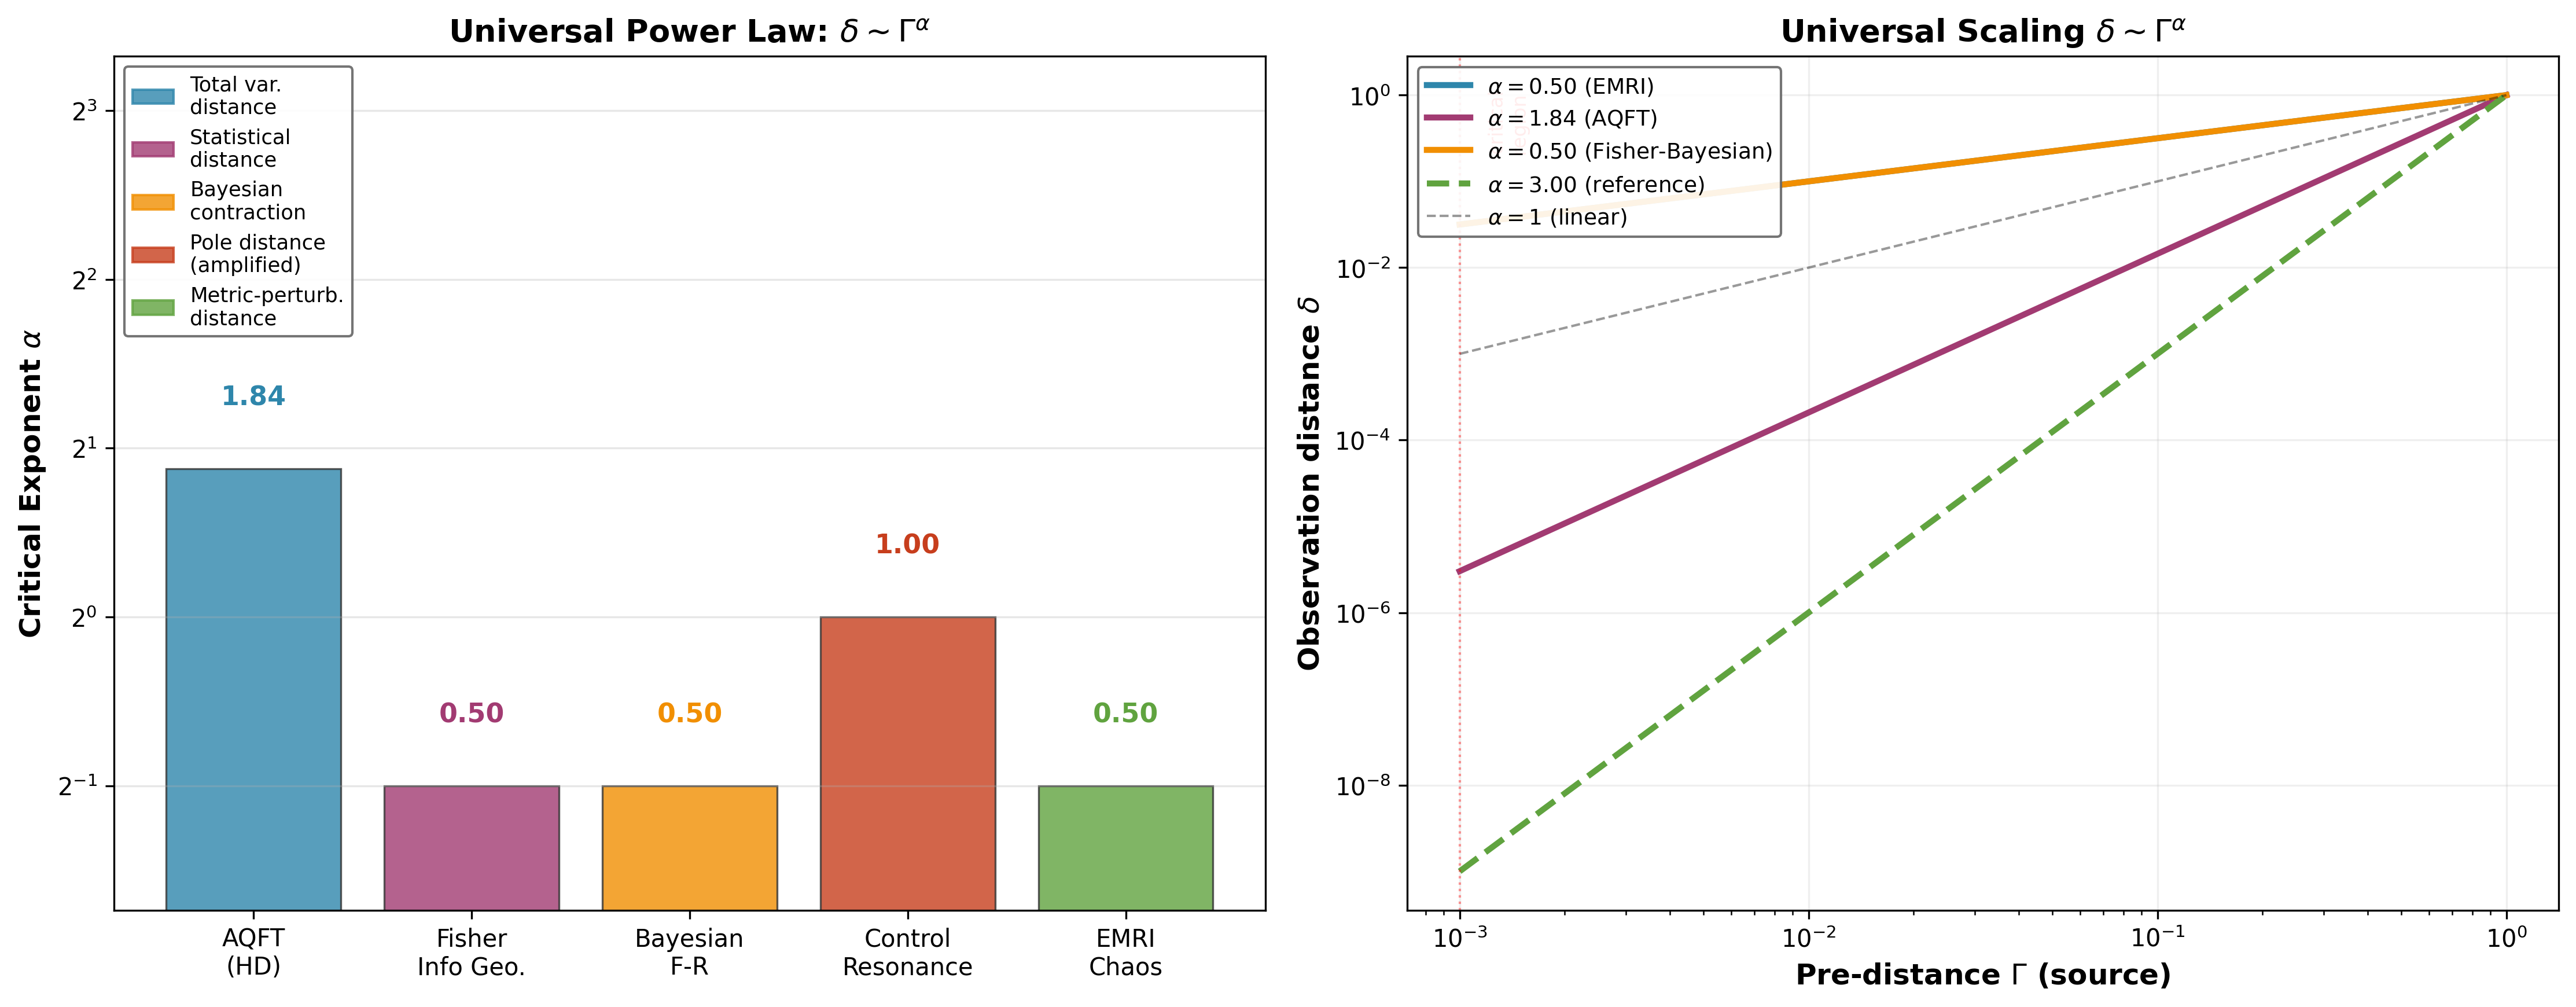
\includegraphics[width=\textwidth]{Fig2-critical-exponents.png}
\caption{Critical exponent comparison across the five DistCat examples. Left: bar chart of \(\alpha\) values on log scale. Right: log-log plots showing the universal scaling law \(\delta \sim \Gamma^\alpha\) — despite different physical origins (AQFT total variation, Fisher information geometry, Bayesian Fisher-Rao, resonance amplification, EMRI chaos), all examples exhibit the same power-law relationship between source pre-distance \(\Gamma\) and observation distance \(\delta\).}
\label{fig:critical-exponents}
\end{figure}

\subsubsection{9.3 Implications for Theory
Unification}\label{implications-for-theory-unification}

If distinct physical theories share the same distance-export structure,
they may be unified as different 0-objects within the same 2-category.
Conjecture 2.6 (observation infeasibility) implies that observational data
alone cannot distinguish between theories in the same distance
equivalence class. Theory choice requires additional criteria:
simplicity of the base category \(\mathbf{C}\), naturalness of the
structure functor \(\mathcal{F}\), or empirical adequacy beyond distance
measurements.

\subsubsection{9.4 Limitation: Discreteness of the GR
Category}\label{limitation-discreteness-of-the-gr-category}

The EMRI example (Example 5) has a \textbf{discrete source category}
\(\mathbf{C}_{\text{EMRI}}\): the Dehnen metrics are analytic in the
parameters \((\rho_s, r_s)\) and \(r\), so an isometric embedding
between two spacetimes requires parameter equality. Consequently,
1-morphisms are only identity morphisms, and all categorical claims
(naturality of \(\eta\), functoriality of morphisms, 2-morphism
composition) are \textbf{vacuously satisfied} for this specific
0-object.

This is not a flaw in the framework --- it is a \textbf{feature of the
distance export principle}. The principle \(\delta = \Phi(\Gamma)\)
holds for EMRI even when the categorical machinery is empty,
demonstrating that the principle is a property of the underlying
geometry of the parameter space, not merely a consequence of categorical
composition. The non-trivial categorical structure (non-discrete
\(\mathbf{C}\), non-vacuous naturality) is exhibited by the other four
examples: D1-grav-waves (AQFT with rich morphism structure between local
algebras), D16+D24 (statistical models with measure-preserving maps),
Bayesian inference (statistical models with stochastic kernels), and D26
(LTI systems with feedback morphisms).

Future work will explore whether \(\mathbf{C}_{\text{EMRI}}\) can be
enlarged to include \textbf{approximately isometric embeddings} (where
\(||\psi^* g_2 - g_1|| < \epsilon\)) or \textbf{local patch embeddings}
(where isometry is required only on a compact region \(U \subset M\)),
which would make the GR example genuinely non-discrete.

\subsubsection{9.5 Open Problems}\label{open-problems}

\begin{enumerate}
\def\labelenumi{\arabic{enumi}.}
\tightlist
\item
  \textbf{Rigorous 2-category proof for EMRI}: The EMRI example
  (Section~\ref{sec:example5-emri}) establishes the key properties of
  the DistCat 2-category: category structure, functoriality of
  $\mathcal{F}$ and $\mathcal{O}$, distance export inequality,
  distance export functor well-definedness, interchange law, and
  structural equivalence to D26. See Propositions~\ref{prop:emri-chaos-resonance}--\ref{prop:emri-d26-dist-eq}.
\item
  \textbf{D1 vs EMRI universality classes}: D1-grav-waves
  ($\alpha \approx 1.84$, log-corrected quadratic) and EMRI
  ($\alpha = 0.5$, homoclinic bifurcation) belong to \textbf{different
  universality classes} with incommensurable exponents. D1's critical
  point is a geometric boundary ($\theta \to 0$ is minimum angular
  separation, not a bifurcation), while EMRI's is a dynamical phase
  transition (KAM-breakup). They share the DistCat 2-categorical
  structure but not numerical exponent classes.
\item
  \textbf{Extension to quantum gravity}: Can the DistCat framework
  accommodate distances derived from quantum gravitational structures
  (e.g., AdS/CFT entanglement entropy)?
\item
  \textbf{Optimal distance export}: Fisher-Rao distance is the unique
  optimal pre-distance among statistical manifolds
  (Amari/Cencov/Chentsov uniqueness theorem). Examples 2 (KL divergence)
  and 3 (Bayesian inference) are statistical manifolds where Fisher-Rao
  optimality applies directly. The other examples use different pre-distances
  (total variation, Lyapunov, geodesic) but follow the same structural
  pattern of distance export. The key result: Fisher-Rao is the unique
  metric making the data processing inequality tight.
\end{enumerate}

\begin{center}\rule{0.5\linewidth}{0.5pt}\end{center}

\subsection{References}\label{references}

\begin{enumerate}
\def\labelenumi{\arabic{enumi}.}
\tightlist
\item
  Hellings, R. \& Downs, G. (1983). Upper bounds on the isotropic
  gravitational radiation background from pulsar timing. \emph{ApJ},
  265, L39.
\item
  Amari, S. (1985). Differential-geometrical methods in statistics.
  \emph{Springer}.
\item
  Hashimoto, K. \& Tanahashi, N. (2017). Universality in chaos of
  particle motion near black hole horizon. \emph{Phys. Rev.~D}, 95,
  024007.
\item
  Peyrard, M. \& Auckly, D. Variational characterization of the Lyapunov
  exponent near Hamiltonian chaos threshold. \emph{Physica D} (2000).
\item
  Das, S., Dalui, S., Lee, B.-H. \& Cai, Y.-F. (2025). EMRI Chaos I:
  Homoclinic orbit and near-horizon chaos. \emph{arXiv:2511.03657}.
\item
  Das, S., Dalui, S., Lee, B.-H. \& Cai, Y.-F. (2025). EMRI Chaos II:
  Chaotic imprints in gravitational waves. \emph{arXiv:2512.04848}.
\item
  Al-Badawi, A., Shaymatov, S. \& Sekhmani, Y. (2025). Schwarzschild
  black hole in galaxies surrounded by a dark matter halo. \emph{JCAP},
  02, 014.
\item
  Kehagias, A. \& Riotto, A. (2024). On the symmetry interpretation of
  the Hellings-Downs curve.
\item
  Maldacena, J., Shenker, S. \& Stanford, D. (2016). A bound on chaos.
  \emph{JHEP}, 08, 106.
\item
  Bombelli, L. \& Calzetta, E. (1992). Chaos around a black hole.
  \emph{Class. Quant. Grav.}, 9, 2573.
\item
  Wiggins, S. (2003). Introduction to Applied Nonlinear Dynamical
  Systems and Chaos. \emph{Springer}.
\item
  Gelfand, I. \& Naimark, M. (1943). On the imbedding of normed rings.
  \emph{Uspekhi Mat. Nauk}, 8, 3-33.
\item
  Lu, C. Extended functorial QFT framework for GW source discrimination
  in pulsar timing arrays. \emph{in preparation} (D1-grav-waves).
\item
  Lu, C. EMRI-D26 resonance mapping: chaos-to-observable
  correspondence. \emph{in preparation} (D26).
\item
  Baez, J. C. \& Lauda, A. D. (2004). Higher-Dimensional Algebra V:
  2-Groups. \emph{Theory Appl. Categ.}, 12, 423, arXiv:math/0307200.
\item
  Lurie, J. (2009). On the Classification of Topological Field
  Theories. \emph{Curr.\ Dev.\ Math.}, 2009, 127.
\end{enumerate}

\end{document}
